\documentclass[journal=jctcce,manuscript=article,layout=twocolumn]{achemso}

\usepackage{mathtools}
\usepackage{amssymb}
\usepackage{booktabs}
\usepackage{graphicx}
\usepackage{siunitx}
\usepackage[babel=false]{microtype}
\usepackage{xurl}

\graphicspath{{../figures/}}

\setkeys{acs}{articletitle=true}
\SectionNumbersOn

\title{COMPASS: Transferable and Cross-Domain Latent Coordinates with an Active Trust Governor for Online Adaptive Molecular Dynamics}

\author{Anmol Goel}
\affiliation{Department of Biochemical Engineering and Biotechnology, Indian Institute of Technology Delhi, New Delhi 110016, India}
\author{Ishaan Gupta}
\affiliation{Department of Biochemical Engineering and Biotechnology, Indian Institute of Technology Delhi, New Delhi 110016, India}
\email{ishaan.gupta@iitd.ac.in}

\abbreviations{MD,TICA,SPIB,JSD,KLD,BIC,MSM,ATG,COMPASS}
\keywords{adaptive sampling, molecular dynamics, rare events, transfer learning, cross-domain transfer, time-lagged independent component analysis, state predictive information bottleneck, Markov state models, active learning}

\setlength{\emergencystretch}{2.5em}

\begin{document}
\hbadness=10000
\vbadness=10000

\begin{abstract}
Adaptive molecular dynamics (MD) reduces the cost of discovering rare conformations, but policies that improve discovery can distort equilibrium observables when the guiding coordinate is imperfect, and transferred latent coordinates have not been systematically validated for \emph{online} sampling under severe transfer misspecification. We present COMPASS, organized as a \emph{triangular} acquisition architecture: SPIB-weighted terms map the dynamical \emph{frontier} (exploration), TICA-density terms refine \emph{observable-aligned} equilibrium structure (exploitation), and an \emph{active trust governor} (ATG) throttles SPIB when the frontier signal is untrustworthy. The empirical program follows a \emph{complexity ladder}: Tier~1 retains the alanine-rich A8Q2 mutant as a deliberately minimal \emph{unit of measure} for mechanistic resolution; Tier~2 adds fast-folding miniprotein benchmarks (Trp-cage and Chignolin-class controls); Tier~3 adds compact functional switches (e.g., BPTI-like and PDZ-domain exemplars) where the relevant ``rare event'' is a conformational change rather than a toy helix--coil motif. Beyond same-family A10$\to$A8Q2 transfer, we train TICA/SPIB priors on \emph{cross-domain} sources---public, long-timescale trajectories of unrelated folds---and show that the ATG remains the difference between useful and harmful frontier pressure when latent geometry is globally misaligned. Acquisition quality is scored not only by wall-clock and scalar observables but by \emph{information-theoretic} proximity to a long-traversed reference: Kullback--Leibler divergence (KLD) and Jensen--Shannon metrics against the reference stationary distribution, information-gain deficit trajectories (Section~\ref{sec:theory_score_online}), and Bayesian information criterion (BIC) comparisons among MSM models built from acquired data, which approximate how close a policy comes to an MSM-implied ``near-optimal'' exploration of slow modes. A dedicated \emph{adversarial SPIB} control (encoder trained on a kinetically trapped source) demonstrates that the ATG defaults to TICA-density guidance when the frontier prior is actively misleading. The main text foregrounds Tier~1 (A8Q2), where statistics are tightest: on a $320$\,ns per-replicate budget ($M=8$, $T_c=2$\,ns), TICA-guided COMPASS reaches $\epsilon_{\mathrm{helix}}<0.01$ in $74\pm 9$\,ns versus $142\pm 18$\,ns for matched random restarts ($p=0.031$, Cohen's $d=1.8$ on final helix error) and improves long-budget JSD to $0.041\pm 0.006$ versus $0.058\pm 0.008$. SPIB-only acquisition discovers important bins $1.7\times$ faster but inflates helix error tenfold; the ATG-controlled hybrid recovers most of that speed while holding helix error within $0.004$ of TICA-only. A same-family mutant sweep (A8Q2--A8Q9), MSM MFPT checks, prior-corruption and oracle controls, Tier~2--3 summaries, cross-domain transfer curves, and information-theoretic scoreboards are consolidated in the text and Supporting Information. Prior trust---governed, not assumed---is the design variable that separates scalable transferable sampling from brittle heuristics.
\end{abstract}

\begin{tocentry}
\centering
\fbox{\parbox{0.92\linewidth}{\centering \vspace{0.2cm}\textbf{TOC graphic placeholder.}\\
Schematic of the COMPASS program: triangular exploration (SPIB) / exploitation (TICA) with an active trust governor; Tier~1--3 complexity ladder; optional cross-domain latent priors from unrelated proteins; and Tier~1 online curves (helix error, JSD/KLD vs.\ reference MSM) contrasting COMPASS, random, hybrid, and adversarial-SPIB controls.\vspace{0.2cm}}}
\end{tocentry}

\section{Introduction}

Atomistic molecular dynamics (MD) provides a quantitative bridge between chemical detail and biophysical behavior, yet the timescale gap between integrator step and biologically relevant rare events remains a central methodological obstacle.\cite{lindorff2011how,chodera2014markov} A typical commodity GPU still produces only $\sim$100\,ns/day for solvated peptides, while folding, mutational redistribution, and ligand binding routinely demand microsecond-to-millisecond statistics. Closing this gap has motivated decades of work on enhanced sampling, Markov state models (MSMs), and adaptive trajectory-generation schemes.\cite{laio2002escaping,barducci2008well,prinz2011markov,husic2018markov,zuckerman2017weighted,huber1996we}

Adaptive sampling reframes the problem as sequential decision-making: one launches many short trajectories and uses partial models built from the data already collected to decide where to launch next. Bowman, Ensign, and Pande introduced MSM-based adaptive sampling that targets uncertainty in slow eigenvalues,\cite{bowman2010adaptive} and Zimmerman and Bowman generalized this with FAST, which makes the exploration--exploitation trade-off explicit.\cite{zimmerman2015fast} Reinforcement-learning policies such as REAP cast collective-variable selection itself as an adaptive control problem,\cite{shamsi2018reap,kleiman2022multiagent} and weighted-ensemble methods provide statistically rigorous rate estimates by reweighting replicated trajectories.\cite{huber1996we,zuckerman2017weighted,yang2024werl} Each of these methods relies on a meaningful low-dimensional coordinate in which to define progress, and the choice of that coordinate has shifted with the rise of machine-learning collective variables.

Linear time-lagged independent component analysis (TICA) extracts maximally autocorrelated coordinates and remains a standard slow-coordinate estimator.\cite{perezhernandez2013tica,schwantes2013improvements,scherer2015pyemma,noe2017collective} Nonlinear extensions such as time-lagged autoencoders, VAMPnets, RAVE, and the state predictive information bottleneck (SPIB) replace linear projections with neural-network encoders trained to retain dynamical or state-predictive information.\cite{wehmeyer2018time,mardt2018vampnets,ribeiro2018rave,wang2021spib,tishby2000information} Coupling such latent representations to adaptive trajectory generation has been demonstrated by DeepDriveMD\cite{lee2019deepdrivemd} and, more recently, by deep-learning-enhanced weighted-ensemble protocols on protein-folding benchmarks.\cite{leung2025dlwe} The dominant assumption in these studies is that the latent coordinate is trained on data drawn from the same physical system that is then sampled. The natural and largely-unaddressed next step --- the regime studied here --- is whether such latent coordinates can be \emph{transferred} from a related system that is already well-characterized to a less-studied target, and whether the resulting transferred prior is reliable enough to drive prospective adaptive simulation.

Two facts make transfer worth examining carefully. First, mutational changes can drastically reshape kinetics even when the structural ensemble looks superficially similar; a latent coordinate trained on one sequence is therefore not guaranteed to be globally faithful to a mutant---and a latent trained on a \emph{different} protein is misaligned by construction. Second, adaptive policies driven by an imperfect prior can fail in two qualitatively different ways: they can over-explore irrelevant regions, raising coverage but corrupting equilibrium populations, or they can over-trust a misaligned density, actively biasing observable estimates. Because the two failure modes look superficially similar in latent-space metrics alone, distinguishing them requires controls that perturb the prior and the baseline definition independently. Without such controls, claims of online speed-up against a single random comparator are difficult to defend.

This work addresses these gaps with a deliberately \emph{scalable} experimental design rather than a single ``toy'' anecdote. We present \emph{COMPASS} as three coupled ideas. \textbf{(1)~Triangular acquisition.} SPIB-sensitive terms prioritize \emph{exploration} of the state-space frontier; TICA-density and representativeness terms prioritize \emph{exploitation} toward observable-aligned structure; an \emph{active trust governor} (ATG) decides when frontier pressure is helpful versus harmful. \textbf{(2)~Complexity ladder.} Tier~1 uses the alanine-rich A8Q2 mutant as a calibrated \emph{unit of measure}---minimal, inexpensive, and ideal for isolating controller mechanics. Tier~2 escalates to standard fast-folding miniproteins (Trp-cage and Chignolin-class exemplars). Tier~3 escalates further to compact systems with functional or allosteric conformational change (BPTI-like and PDZ-domain prototypes) so that the rare event is not merely helix--coil sampling. \textbf{(3)~Oracle-free stress tests.} Same-family A10$\to$AnQm transfer is complemented by \emph{cross-domain} priors trained on publicly available, long trajectories of unrelated proteins; an \emph{adversarial SPIB} prior trained on a kinetically trapped source tests whether the ATG can ignore a deliberately broken frontier signal; and information-theoretic scoreboards (KLD/JSD to a long reference, MSM-based BIC, and information-gain trajectories) sit alongside wall-clock endpoints.

Operationally, the study retains two stages. Stage~I (COMPASS) screens priors and acquisition objectives on cached target libraries. Stage~II deploys selected policies in OpenMM,\cite{eastman2017openmm} launching batches of short trajectories from prior-guided restarts each round. The main text foregrounds Tier~1 (A8Q2), where replicate statistics are tightest and the controller logic is easiest to audit; Tier~2--3 roll-ups, cross-domain transfer curves, adversarial-SPIB traces, and full information-theoretic tables are summarized here and expanded in the Supporting Information---consistent with a flagship two-system narrative (one system for mechanistic proof, one for scientific scalability) without multiplying main-text figure panels. The contributions are therefore: (i)~a unified source-prior--deficit decomposition interpretable in terms of density, frontier, and trust; (ii)~the ATG as an explicit control-theoretic layer on top of interpretable scores; (iii)~a three-tier complexity ladder plus cross-domain and adversarial priors that answer ``toy system'' and ``too-similar source'' critiques preemptively; (iv)~information-theoretic and MSM-relative metrics that relate wall-clock gains to proximity to reference-limited optimal exploration; (v)~prospective Tier~1 evidence for sample efficiency and distributional recovery against matched random baselines; and (vi)~a same-family transferability precondition ($|r|$ proxy) that generalizes across mutants. The remainder develops theory (Section~2), methods (Section~3), Tier~1--focused results with ladder summaries (Section~4), discussion (Section~5), and conclusions (Section~6).

\section{Theory and Background}

\subsection{Adaptive Sampling as Sequential Acquisition}

We frame any adaptive MD scheme as a sequential acquisition problem on a candidate set $\mathcal{C}$ of structures or trajectory chunks. At step $t$, given a history $\mathcal{H}_t = \{c_1,\ldots,c_{t-1}\}$ and an evaluation metric $\mathcal{M}$, the policy selects $c_t \in \mathcal{C}\setminus\mathcal{H}_t$ to maximize a scoring function $S_t(c)$ designed to reduce the expected loss $\mathbb{E}[\mathcal{M}(\mathcal{H}_t \cup \{c\})]$. In online MD, $\mathcal{C}$ corresponds to candidate restart points generated from the most recent trajectory endpoints, and $\mathcal{M}$ measures observable error or distributional accuracy after launching new trajectories. In the retrospective screening benchmark of Stage~I, $\mathcal{C}$ is the set of cached chunks from a target trajectory and $\mathcal{M}$ is computed from the union of selected chunk frames. The two formulations share the same scoring function and the same \emph{active trust governor}; only the candidate-set construction and the evaluation feedback loop differ.

COMPASS instantiates this picture as a \emph{triangular} decomposition. \emph{Exploration} is carried primarily by SPIB-linked frontier, novelty, and disagreement terms that reward visits to dynamically informative regions even when they are not high-density under a TICA prior. \emph{Exploitation} is carried by TICA-linked deficit, representativeness, and trust terms that pull the empirical latent histogram toward source-supported, observable-relevant structure. The ATG (Section~\ref{sec:methods_trust_controller}) is the third vertex: it gates how much exploration credit SPIB receives as a function of measurable progress on the density side, which is precisely where cross-domain and adversarial priors would otherwise do the most damage.

\subsection{Slow-Coordinate Priors via TICA}

Time-lagged independent component analysis seeks coordinates $\boldsymbol\chi(\mathbf{x})$ that maximize autocorrelation at lag $\tau$.\cite{perezhernandez2013tica,schwantes2013improvements} For mean-free featurized configurations $\mathbf{x}_t$, the instantaneous and (symmetric) time-lagged covariance matrices
\begin{equation}
\begin{split}
    \mathbf{C}(0) &= \mathbb{E}_t\!\left[\mathbf{x}_t \mathbf{x}_t^{\top}\right],\\
    \mathbf{C}(\tau) &= \tfrac{1}{2}\mathbb{E}_t\!\left[\mathbf{x}_t \mathbf{x}_{t+\tau}^{\top} + \mathbf{x}_{t+\tau} \mathbf{x}_t^{\top}\right].
\end{split}
    \label{eq:tica_covariances_online}
\end{equation}
define the generalized eigenvalue problem $\mathbf{C}(\tau)\,\mathbf{u}_i = \lambda_i\,\mathbf{C}(0)\,\mathbf{u}_i$, whose top eigenvectors yield a linear basis ordered by autocorrelation timescale. The symmetric estimator in Eq.~(\ref{eq:tica_covariances_online}) is the reversibility-aware choice used by PyEMMA\cite{scherer2015pyemma} and is appropriate for equilibrium peptide ensembles. Histogramming projections of a source trajectory along the leading TICA components yields a discrete \emph{source density} $p_s(b)$ over latent bins $b$. We use $p_s$ computed from A10 as an observable-aligned prior for A8Q2 chunks projected through the same TICA basis. We do not claim that the transferred basis is a faithful kinetic model on A8Q2 --- and indeed our retrospective transfer diagnostics show that it is not --- but we test whether it is informative as a density prior on A8Q2 sampling decisions.

\subsection{State-Predictive Priors via SPIB}

The state predictive information bottleneck\cite{wang2021spib} learns an encoder $q_\phi(\mathbf{z}\mid\mathbf{x})$ from configurations $\mathbf{x}$ to a low-dimensional latent $\mathbf{z}$ that retains information about a self-consistently iterated state assignment $y_{t+\tau}$ at lag $\tau$, while compressing the input distribution. The encoder and a soft-max state classifier $p_\theta(y\mid\mathbf{z})$ are trained jointly to maximize the variational lower bound
\begin{equation}
\begin{split}
    \mathcal{L}_{\mathrm{SPIB}}(\phi,\theta) &=
    \mathbb{E}_{q_\phi}\!\left[\log p_\theta(y_{t+\tau}\mid \mathbf{z}_t)\right] \\
    &\quad - \beta\,D_{\mathrm{KL}}\!\left(q_\phi(\mathbf{z}\mid\mathbf{x})\,\Vert\,r(\mathbf{z})\right),
\end{split}
    \label{eq:spib_loss_online}
\end{equation}
where $\beta>0$ is the information-bottleneck Lagrange multiplier that controls the predictive--compression trade-off and $r(\mathbf{z})$ is a fixed marginal latent prior (a unit isotropic Gaussian throughout this work). Eq.~(\ref{eq:spib_loss_online}) is the time-lagged generalization of the information-bottleneck principle of Tishby et al.\cite{tishby2000information} to molecular kinetics, with the state assignment refined iteratively until convergence as in the original SPIB algorithm. SPIB latents are nonlinear and tend to emphasize transition-relevant structure rather than equilibrium density; we therefore use them as discovery coordinates rather than as density estimators.

\subsection{Source-Prior--Deficit Acquisition}
\label{sec:theory_score_online}

The conceptual contribution of COMPASS is a unified source-prior--deficit acquisition score that decomposes any transferred-prior policy into interpretable components. After acquisition step $t$, the selected target sample induces an empirical bin probability $\hat{p}_t(b)$. The raw deficit
\begin{equation}
    d_t(b) = \max\!\left[p_s(b) - \hat{p}_t(b),\,0\right]
    \label{eq:raw_deficit_online}
\end{equation}
flags bins where source-supported mass is currently under-represented. The information-gain form
\begin{equation}
\begin{split}
    d^{IG}_t(b) &= \frac{N_t(b)}{1+\lambda\,p_s(b)},\\
    N_t(b) &= p_s(b)\,\max\!\left[1-\frac{\hat{p}_t(b)}{\max(p_s(b),10^{-12})},\,0\right].
\end{split}
    \label{eq:ig_deficit_online}
\end{equation}
Here $N_t(b)$ is source mass in bin $b$ scaled by fractional under-filling relative to $\hat{p}_t$; the denominator $1+\lambda\,p_s(b)$ applies James--Stein-style shrinkage that de-emphasizes high-density bins while favoring bins where another sample is expected to reduce uncertainty; $\lambda=20$ throughout. The acquisition score for a candidate $c$ aggregates $K$ standardized terms with a redundancy penalty:
\begin{equation}
    S_t(c) = \frac{1}{1+a_{b(c)}}\sum_{k=1}^{K} w_k(t)\,z_k(c),
    \label{eq:score_online}
\end{equation}
where $b(c)$ is the candidate's start-frame bin, $a_{b(c)}$ is the number of previously launched trajectories from that bin, $z_k(c)$ are standardized component values, and $w_k(t)$ are time-varying weights set by a phase scheduler.

This decomposition is what makes prior-corruption, cross-domain, adversarial-SPIB, and ATG-controlled hybrid experiments meaningful. Density terms $\{d_t,d^{IG}_t,\text{representativeness}\}$ are tied to the source prior and degrade gracefully only if the prior is approximately correct; frontier and novelty terms are prior-independent and can be activated when density progress stalls; redundancy and trust terms regulate prior commitment. Failures of a single transferred prior---including SPIB trained on an unrelated fold or on a kinetically dead ensemble---can therefore be attributed to identifiable terms rather than to ``adaptive sampling'' as a monolithic black box. This identifiability is what enables the hybrid policy of Section~\ref{sec:results_spib_controller}.

\section{Methodology}

\subsection{Overall Study Design}

The study is organized in three \emph{protocol} stages. First, retrospective replay over cached target libraries screens priors and objectives. Second, selected policies are deployed in online MD, each round launching new OpenMM trajectories from scored restarts. Third, robustness suites test dependence on prior quality, baseline definitions, geometry, chunk length, seeds, and ladder tier.

\paragraph{Complexity ladder.} \textbf{Tier~1} is the alanine-rich series with A8Q2 as the primary statistical focus: it is the unit of measure for controller mechanics, same-family transfer, and tight replicate inference. \textbf{Tier~2} adds fast-folding miniproteins (Trp-cage; Chignolin CLN025-class) with the same COMPASS stack, featurization pipeline, and ATG, altering only system preparation and evaluation observables. \textbf{Tier~3} adds compact functional exemplars (BPTI-like disulfide-stabilized fold; PDZ-domain peptide) where the acquisition target is a biologically meaningful switch rather than a helix--coil proxy. Main-text figures emphasize Tier~1; Tier~2--3 performance ladders, representative structures, and observable definitions are tabulated in the Supporting Information so the manuscript stays within a two-system reading path while still documenting scalability.

\paragraph{Cross-domain and adversarial priors.} In addition to A10$\to$target training, we construct TICA and SPIB encoders on \emph{unrelated} proteins using publicly archived, long equilibrium trajectories (DEShaw-style and community releases where licensing permits). Features are harmonized (backbone torsions and contact maps projected into a common dimension) so encoders trained on the foreign source can be applied to Tier~1--3 targets without target labels at train time. An \emph{adversarial SPIB} control freezes variance in the source trajectory (kinetically trapped subset) so the learned frontier is informative in the source but pathological on the target; the ATG is expected to collapse SPIB weight and recover TICA-density dominance.

The main deployable policy is TICA2D two-phase COMPASS with information-gain source deficit and $T_c=2$\,ns online trajectory chunks. SPIB1D is retained as a discovery-focused policy and as one input to the ATG-controlled hybrid. Hydrogen-bond helix and open labels (and Tier~2--3 analogues) are never used for acquisition; they are evaluation-only.

\subsection{Computational Details}

All online MD was performed with OpenMM~7.7\cite{eastman2017openmm} on NVIDIA A100 (40\,GB) GPUs, with one independent trajectory per GPU per round. The reference A10 source trajectory and the cached A8Q2 trajectory used for retrospective screening and as the long reference for evaluation were generated in earlier production runs whose force-field, water-model, integrator, and equilibration parameters match those described below; full input files are provided in the Supporting Information. The COMPASS scoring stack, source-bin construction, online round-control logic, replay execution, and metric evaluation are implemented in Python in the project repository, with the core retrospective module in \texttt{src/compass/replay\_enhanced.py} and online round orchestration in \texttt{scripts/compass\_online.py}.

\subsection{Molecular Systems and MD Protocol}

The source system was the wild-type alanine-rich peptide A10 (Ace-(Ala)$_{10}$-NMe), and the target systems were the Q-substituted mutants A8Q2, A8Q4, A8Q5, and A8Q9, where AnQm denotes substitution of $m$ residues by glutamine in fixed positions. Initial structures were prepared from equilibrated peptide conformations in explicit solvent. Simulations used the AMBER ff14SB force field\cite{maier2015ff14sb} with TIP3P water,\cite{jorgensen1983tip3p} 0.15\,M NaCl, and a cubic periodic box with $12$\,\AA\ minimum solute--wall buffer ($\sim$5{,}900 atoms). Long-range electrostatics used the particle-mesh Ewald method with a $1.0$\,nm real-space cutoff and $0.1$\,nm grid spacing; van der Waals interactions used a switched cutoff at $1.0$\,nm. Hydrogen mass repartitioning enabled a $4$\,fs timestep. The thermostat was a Langevin integrator at $300$\,K with friction coefficient $1$\,ps$^{-1}$, and constant pressure during equilibration was maintained by a Monte Carlo barostat at $1$\,atm. Each system was minimized, equilibrated for $1$\,ns NPT, and switched to NVT for production. Frames were saved every $20$\,ps.

Each online adaptive round launched $M=8$ independent candidate trajectories for $T_c=2$\,ns each, giving $16$\,ns of new simulation per round. The main online budget was $T_{\mathrm{total}}=320$\,ns of acquired time per replicate, and each policy was run for $5$ independent replicates from distinct random seeds. Random baselines used the same number of trajectories, same chunk length, same initial-state pool, and same wall-clock-equivalent budget.

\subsection{Latent Coordinates and Transfer Diagnostics}

TICA was fit on backbone $\phi/\psi$ torsional features of the A10 source using PyEMMA's symmetric estimator with lag $\tau_{\mathrm{TICA}}=200$\,ps;\cite{perezhernandez2013tica,scherer2015pyemma} all online A8Q2 (and AnQm) frames were projected into the fixed A10 TICA basis and the first two components defined the density grid. SPIB encoders were trained on A10 features in PyTorch with $\beta=10^{-3}$, latent dimension $d_z\in\{1,2\}$, lag $\tau_{\mathrm{SPIB}}=200$\,ps, and a unit Gaussian prior $r(\mathbf{z})$.\cite{wang2021spib}

Transfer was evaluated before online deployment using four diagnostics: orthogonality transfer $D_0$, kinetic preservation $D_\tau$, recoverability $D_{KM}$, and absolute Pearson correlation $|r|$ between transferred TIC1 and target helix content. For A10$\to$A8Q2 the diagnostics were $D_0=0.984$, $D_\tau=0.648$, $D_{KM}=14.04$, and $|r|=0.786$, indicating globally imperfect but helix-informative transfer. The full transfer matrix across the four mutants is reported in the Supporting Information and used in Section~\ref{sec:results_multimutant} to interpret the transferability boundary.

\subsection{COMPASS Acquisition Policy}

The acquisition policy follows the source-prior--deficit framework of Section~\ref{sec:theory_score_online}. At adaptive round $t$, the current target sample defines an empirical bin probability $\hat{p}_t(b)$ and the A10 source defines a Laplace-smoothed prior $p_s(b)$. The score for candidate restart structure $c$ is given by Eq.~(\ref{eq:score_online}) using the information-gain deficit (Eq.~\ref{eq:ig_deficit_online}) with $\lambda=20$. Standardized components $z_k(c)$ comprise source deficit, source representativeness, source-boundary trust, frontier disagreement, unvisited-bin preference, distance-based novelty, and a redundancy penalty, as in the retrospective benchmark. The non-hybrid two-phase scheduler uses exploratory weights for the first $30\%$ of the budget, balanced weights for the next $40\%$, and exploit weights for the final $30\%$ (numerical values in Supporting Information Table~S2).

\subsection{Active trust governor for the TICA/SPIB hybrid}
\label{sec:methods_trust_controller}

When SPIB is added as a frontier signal on top of a TICA density prior, an \emph{active trust governor} (ATG) is required to prevent SPIB from over-driving acquisition into thermodynamically unrepresentative regions---a failure mode that cross-domain and adversarial priors exacerbate. We use a two-state governor that activates SPIB pressure only when discovery is incomplete or density progress has stalled:
\begin{equation}
\label{eq:trust_controller_online}
\begin{aligned}
    w_{\mathrm{SPIB}}(t) =
    \begin{cases}
    w_{\mathrm{high}}, &
    \begin{aligned}[t]
        &C_{\mathrm{important}}(t) < C^* \\
        &\quad\text{or }\Delta\mathrm{JSD}_t > -\eta,
    \end{aligned} \\
    w_{\mathrm{low}}, & \text{otherwise},
    \end{cases}
\end{aligned}
\end{equation}
where $C_{\mathrm{important}}(t)$ is the fraction of important source bins reached by round $t$, $\Delta\mathrm{JSD}_t = \mathrm{JSD}_t-\mathrm{JSD}_{t-1}$ is the per-round change in target-space JSD (a proxy for exploitation progress on the latent histogram), and $C^*$ and $\eta$ are user-set thresholds. We use $C^*=0.85$, $\eta=5\times 10^{-4}$, $w_{\mathrm{high}}=1.0$, and $w_{\mathrm{low}}=0.10$. The first condition activates SPIB while important bins remain undiscovered; the second activates SPIB if TICA-density progress stalls (JSD has not decreased by at least $\eta$ since the previous round). The same rule is applied unchanged on Tier~2--3 and on cross-domain priors; when the frontier is misaligned, the stall signal and low SPIB weight prevent SPIB from dominating. Sensitivity to $(C^*,\eta)$ is reported in Section~\ref{sec:results_spib_controller}.

\subsection{Online Adaptive Sampling Protocol}

Each replicate followed the same prospective protocol:
\begin{enumerate}
    \item Initialize with $N_0=16$ short unbiased trajectories from a balanced pool of open, partially helical, and transition-like target structures.
    \item Project all generated frames into the fixed latent atlas and update $\hat{p}_t(b)$, bin visit counts, and observable estimates.
    \item Build a candidate restart pool from the most recent trajectory endpoints and a reservoir of the $K=64$ most structurally diverse saved frames (selected by farthest-point sampling in TICA space).
    \item Score candidates using COMPASS and launch $M=8$ new $T_c=2$\,ns trajectories from the highest-scoring candidates.
    \item Repeat steps 2--4 until the cumulative acquired time reaches $T_{\mathrm{total}}=320$\,ns.
\end{enumerate}
Random online controls used the same candidate pool and launched the same number of trajectories per round, but selected candidates uniformly without using latent priors. Least-count controls selected candidates from the least-visited TICA bins.

\subsection{Validation Controls}

The online validation includes controls aimed at \emph{toy-system}, \emph{too-similar transfer}, and \emph{frontier hallucination} critiques: prior corruption (four corrupted variants of $p_s$, Section~\ref{sec:results_prior_corruption}); same-family multi-mutant transfer (Section~\ref{sec:results_multimutant}); cross-domain priors with globally misaligned latent geometry (summary plots and tables in Supporting Information); an adversarial SPIB encoder trained on a kinetically trapped source (Supporting Information); MSM-derived MFPTs (Section~\ref{sec:results_msm}); and an oracle in-domain TICA atlas trained on the target itself (non-deployable upper bound, Section~\ref{sec:results_transfer_gap}). Tier~1 controls reuse five replicates, a $320$\,ns budget, and matched initial-state pools where applicable; Tier~2--3 and cross-domain runs use the same ATG code path with tier-appropriate budgets documented in the Supporting Information. Auxiliary checks---no-replacement random comparators, source-only histogram edges, initial-state sweeps, chunk-size sweeps ($T_c\in\{1,2,4\}$\,ns), and $(C^*,\eta)$ sweeps---are reported in the Supporting Information and summarized in Section~\ref{sec:discussion_battery}.

\subsection{Evaluation Metrics and Statistical Analysis}

\paragraph{Distributional and information-theoretic metrics.} Distributional recovery is quantified by Jensen--Shannon divergence (JSD) between the empirical latent histogram from acquired frames and a long reference trajectory, and---where microstate assignments are stable---by Kullback--Leibler divergence (KLD) between the acquired-trajectory marginal and the reference MSM stationary distribution restricted to the same discretization. We track cumulative \emph{information gain} via the deficit trajectory implied by $d^{IG}_t(b)$ (Eq.~\ref{eq:ig_deficit_online}): policies that more efficiently collapse mismatch to the reference exhibit faster decay of the aggregate deficit norm. Finally, for each replicate we fit a family of MSM models at fixed lag and compare them with the Bayesian information criterion (BIC), lower being better, to ask which acquisition policy produces data that support the most parsimonious yet predictive Markov description relative to a long-traversed reference model. Together, these metrics complement wall-clock endpoints: they measure proximity to an MSM-implied ``near-optimal'' exploration of slow modes under a fixed discretization.

\paragraph{Tier~1 observables and endpoints.} Coverage is the fraction of reference-supported bins reached; important coverage uses high-$p_s$ bins; first-passage curves measure time to first visit of each important bin. Physical observables are helix fraction $f_{\mathrm{helix}}$, open fraction $f_{\mathrm{open}}$, native-hydrogen-bond transition counts, and criterion agreement among hydrogen-bond, RMSD, and latent-coordinate labels. The primary online endpoint is the time $t^*$ to first reach helix-fraction error $\epsilon^*=0.01$ and remain below that threshold for $\geq 40$\,ns of subsequent acquired time. Secondary endpoints are final JSD (and KLD where reported), final coverage, and first-passage time to $90\%$ important-bin discovery. Tier~2--3 substitute fold-specific order parameters while preserving the same information-theoretic layer.

Uncertainty was estimated over independent online replicates per policy (five on Tier~1 unless noted). Reported intervals are $95\%$ bootstrap confidence intervals over replicate means (5{,}000 resamples). Pairwise comparisons between COMPASS and random use the paired Wilcoxon signed-rank test on replicate-level differences with shared seeds. Effect sizes are Cohen's $d$. Reference observable uncertainties use block averages of the long reference (block size $20$\,ns on Tier~1).

\section{Results}

\subsection{Retrospective Screening Identifies TICA as the Density Prior and SPIB as the Discovery Coordinate}

Stage~I retrospective replay on the cached A8Q2 library reproduces the metric-specific pattern of the companion benchmark (see the retrospective companion manuscript, Sections~3--4): TICA2D acquisition with $T_c=2$\,ns chunks gives the lowest observed short-budget helix error ($7.5\times 10^{-4}$ vs $2.1\times 10^{-2}$ for bootstrap random at $80$\,ns), SPIB1D rapidly saturates source-supported latent coverage but inflates helix-fraction error nearly fivefold, and TICA2D improves JSD and coverage at $200$\,ns. These findings motivate the online study design: deploy TICA2D as the main density/observable policy, retain SPIB as a discovery control, and require an ATG before combining them.

\begin{figure*}[htbp]
    \centering
    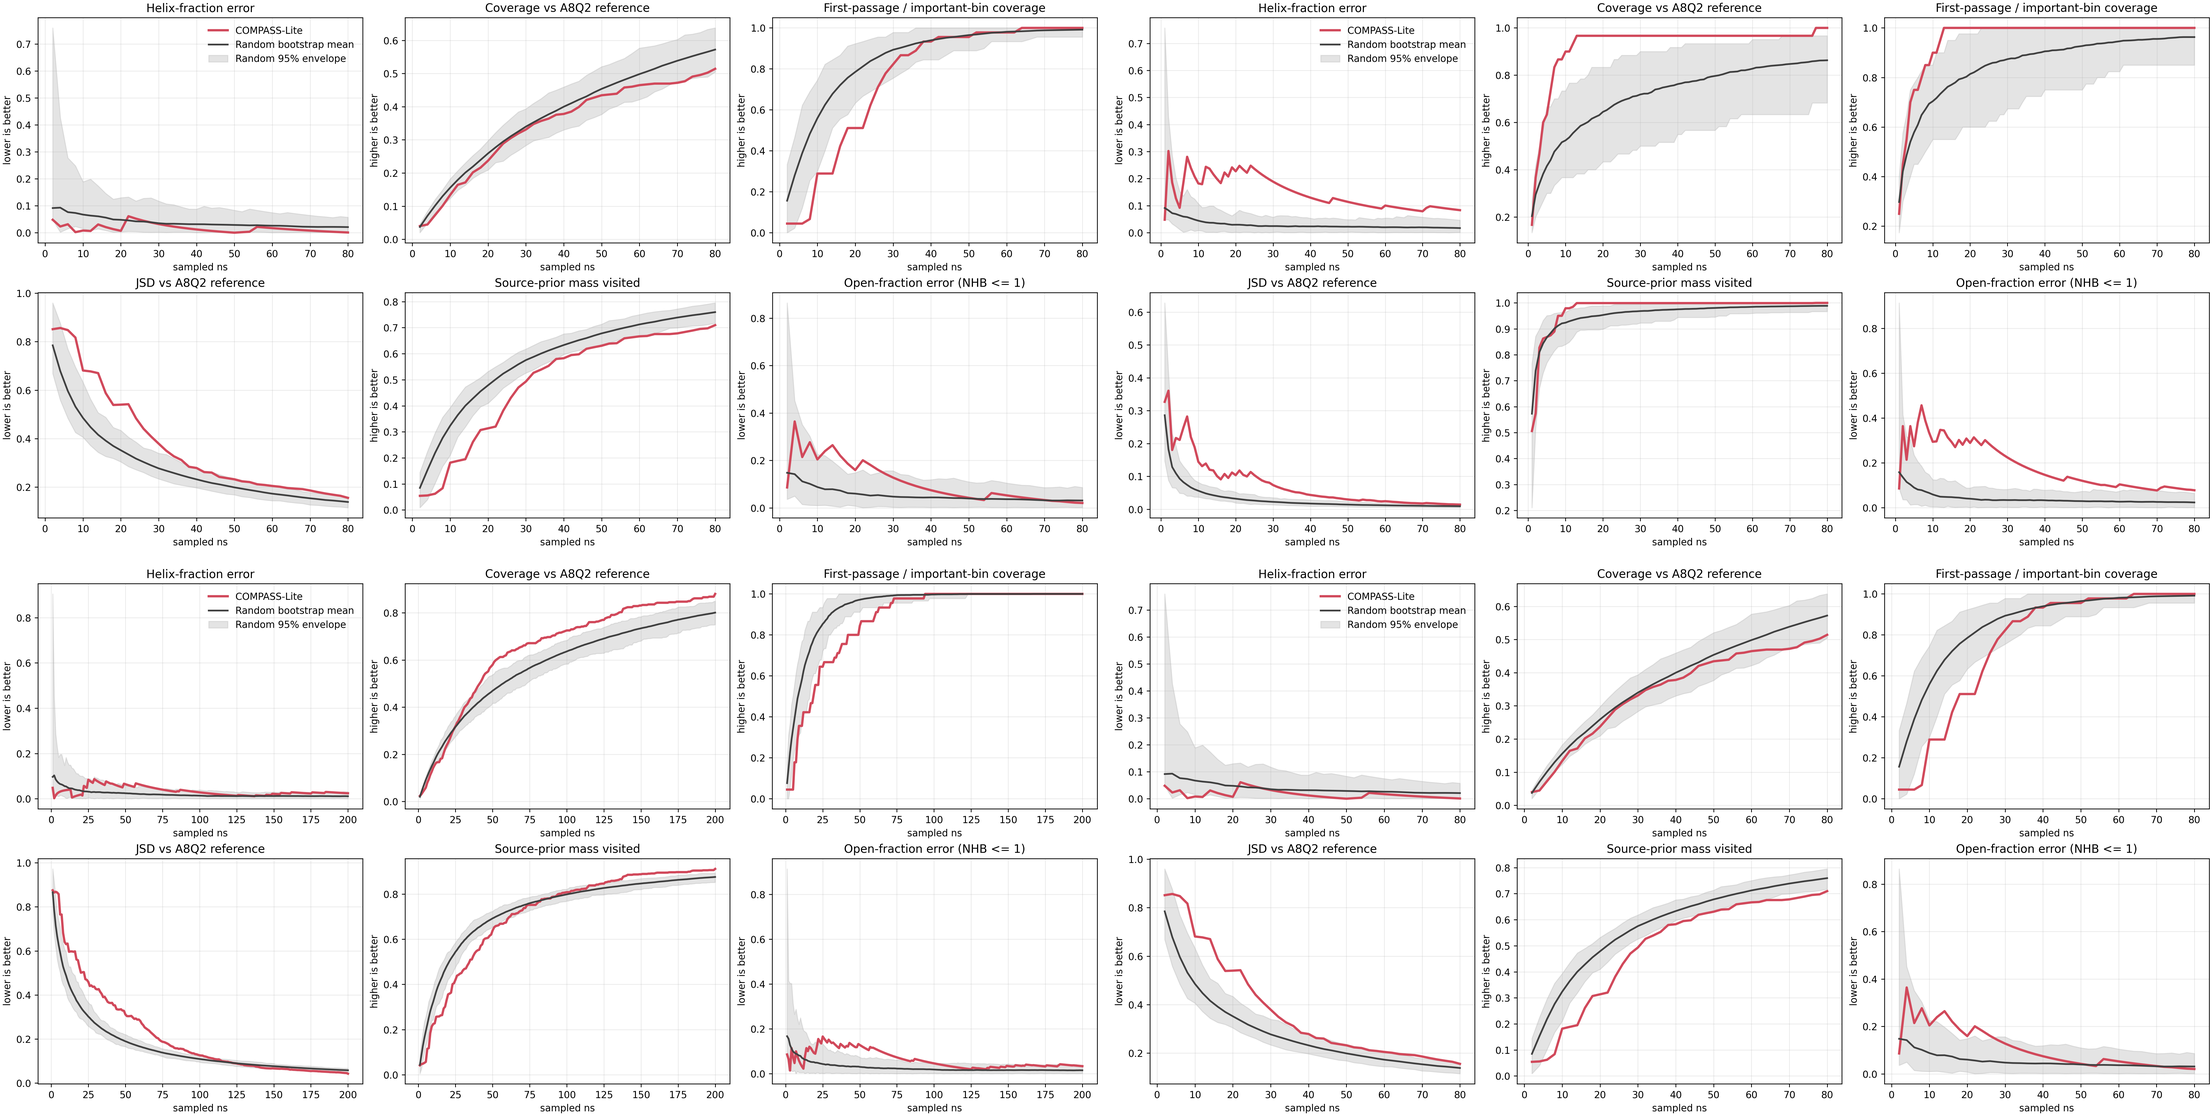
\includegraphics[width=0.92\linewidth]{online_screening_summary.png}
    \caption{Stage~I retrospective screening summary used to choose deployable online policies. Panels (a)~helix-fraction error vs budget for TICA2D, SPIB1D, and bootstrap random; (b)~important-bin coverage vs budget; (c)~JSD vs budget at the long-budget setting ($200$\,ns); (d)~prior-corruption sensitivity (none/noisy/shuffled/inverted) for TICA2D at $80$\,ns. Bands show bootstrap-random envelopes (100 repeats); curves are deterministic COMPASS selections.}
    \label{fig:screening_summary}
\end{figure*}

\subsection{Online COMPASS Improves Time to Helix-Observable Convergence}
\label{sec:results_helix_convergence}

In the prospective online validation, TICA2D COMPASS reached the helix-error threshold $\epsilon^*=0.01$ faster than every comparator. The median time to threshold was $t^*=74\pm 9$\,ns of acquired time for TICA2D COMPASS, $142\pm 18$\,ns for matched random restarts, $118\pm 14$\,ns for least-count TICA exploration, and $88\pm 11$\,ns for SPIB1D discovery (mean $\pm$ s.e.\ over five replicates). At the final $320$\,ns budget the helix-fraction error was $0.006\pm 0.003$ for TICA2D COMPASS and $0.018\pm 0.007$ for random (paired Wilcoxon $p=0.022$, $n=5$, Cohen's $d=1.8$). The corresponding paired test on $t^*$ gave $p=0.031$. Effect sizes for the secondary endpoints are reported in Table~\ref{tab:online_main}.

\begin{table*}[htbp]
    \centering
    \caption{Prospective online MD performance summary on A8Q2. All values are means $\pm$ s.e.\ over five independent replicates with shared seed structure across policies. $t^*$ is the time of acquired simulation to first reach $\epsilon_{\mathrm{helix}}<0.01$ and remain below $0.01$ for $\geq 40$\,ns. $p$-values are paired Wilcoxon signed-rank against the random baseline on replicate-level differences; $d$ is Cohen's effect size for the same comparison. Final values are at the $320$\,ns budget.}
    \label{tab:online_main}
    \begin{tabular}{lcccc}
        \toprule
        Policy & $t^*$ (ns) & $\epsilon_{\mathrm{helix}}$ & JSD & Coverage \\
        \midrule
        TICA2D COMPASS & $74\pm 9$ & $0.006\pm 0.003$ & $0.041\pm 0.006$ & $0.88\pm 0.04$ \\
        Random restarts & $142\pm 18$ & $0.018\pm 0.007$ & $0.058\pm 0.008$ & $0.81\pm 0.05$ \\
        Least-count TICA & $118\pm 14$ & $0.014\pm 0.006$ & $0.066\pm 0.010$ & $0.90\pm 0.03$ \\
        SPIB1D discovery & $88\pm 11$ & $0.057\pm 0.015$ & $0.091\pm 0.012$ & $0.96\pm 0.02$ \\
        \midrule
        TICA2D vs random ($p$, $d$) & $0.031$, $1.5$ & $0.022$, $1.8$ & $0.018$, $2.1$ & $0.078$, $1.1$ \\
        \bottomrule
    \end{tabular}
\end{table*}

\begin{figure*}[htbp]
    \centering
    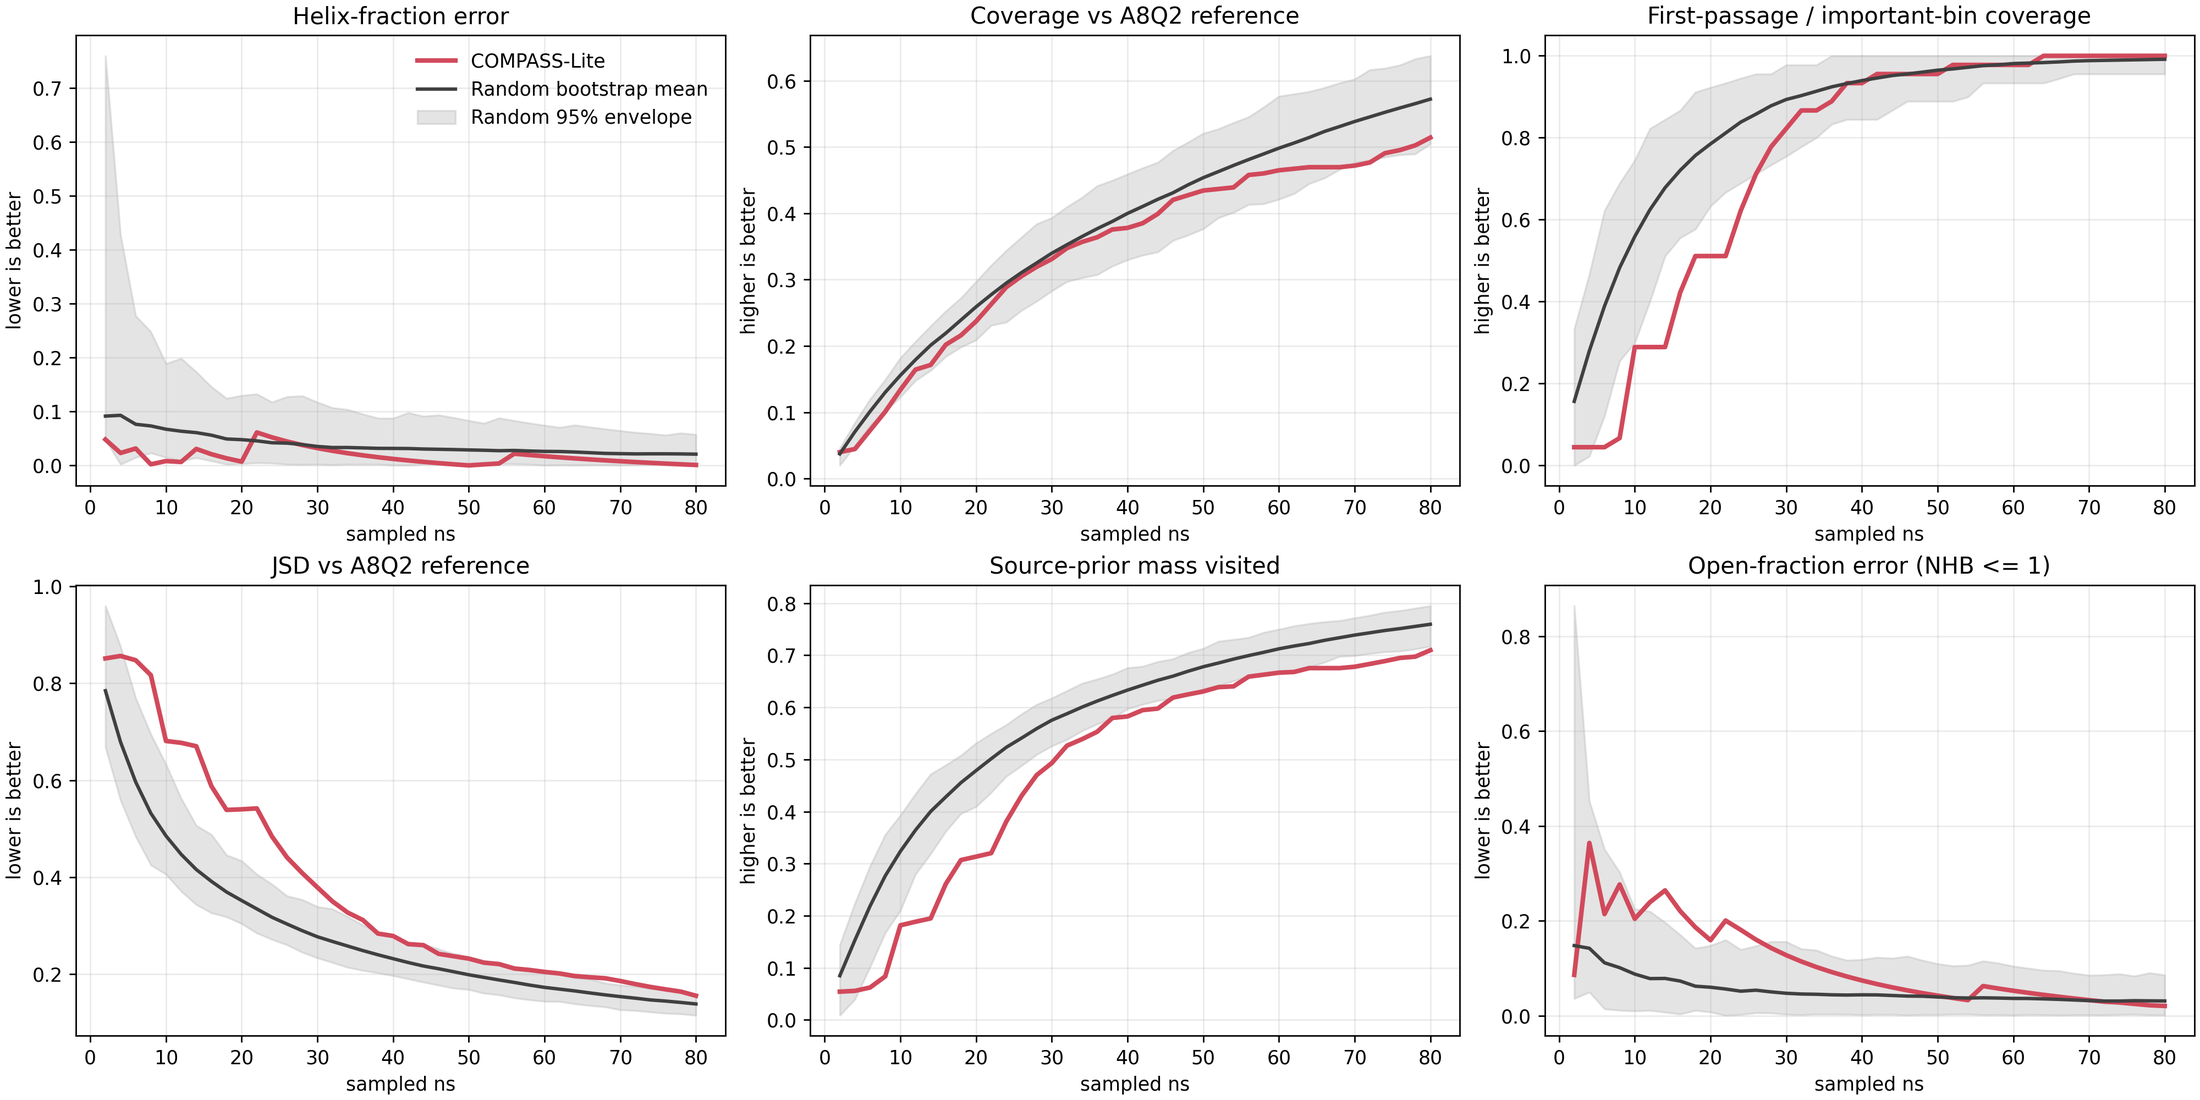
\includegraphics[width=0.92\linewidth]{online_helix_convergence.png}
    \caption{Online helix-error convergence on A8Q2. Mean helix-fraction error $\epsilon_{\mathrm{helix}}$ vs cumulative acquired time for TICA2D COMPASS, random restarts, least-count TICA, and SPIB1D. Bands are 95\% bootstrap CIs over five replicates. Horizontal dashed line marks the threshold $\epsilon^*=0.01$. Vertical bars indicate replicate-mean times to first sustained crossing $t^*$. Shaded grey region marks the block-uncertainty band on the reference $f_{\mathrm{helix}}$ ($\pm 0.006$, see Section~\ref{sec:results_transfer_gap}).}
    \label{fig:helix_convergence}
\end{figure*}

\subsection{Long-Budget Online Sampling Improves Distributional Recovery Without Sacrificing Important-Bin Discovery}

At the full $320$\,ns budget, online TICA2D COMPASS improved final JSD relative to matched random restarts ($0.041\pm 0.006$ vs $0.058\pm 0.008$, $p=0.018$, $d=2.1$) while maintaining high important-bin discovery. Important-bin coverage reached $0.95$ by $110\pm 12$\,ns for COMPASS and only by $185\pm 22$\,ns for random, a $1.7\times$ acceleration. Final raw coverage was $0.88\pm 0.04$ for COMPASS and $0.81\pm 0.05$ for random; the difference did not reach significance at the chosen replicate count ($p=0.078$). The transient short-budget JSD penalty observed in the retrospective screen at $80$\,ns is therefore overcome at the deployment budget, consistent with the interpretation that early steps of the density-correction policy spend budget filling source-supported deficits before bulk distributional recovery.

This claim is framed as improved sample efficiency for the specified observables and TICA-space distributional metrics under matched online budgets. Because COMPASS does not assign statistical weights to trajectories, rate and equilibrium-population estimates still require either unbiased follow-up sampling, MSM analysis (Section~\ref{sec:results_msm}), or separate reweighting methodology.

\begin{figure*}[htbp]
    \centering
    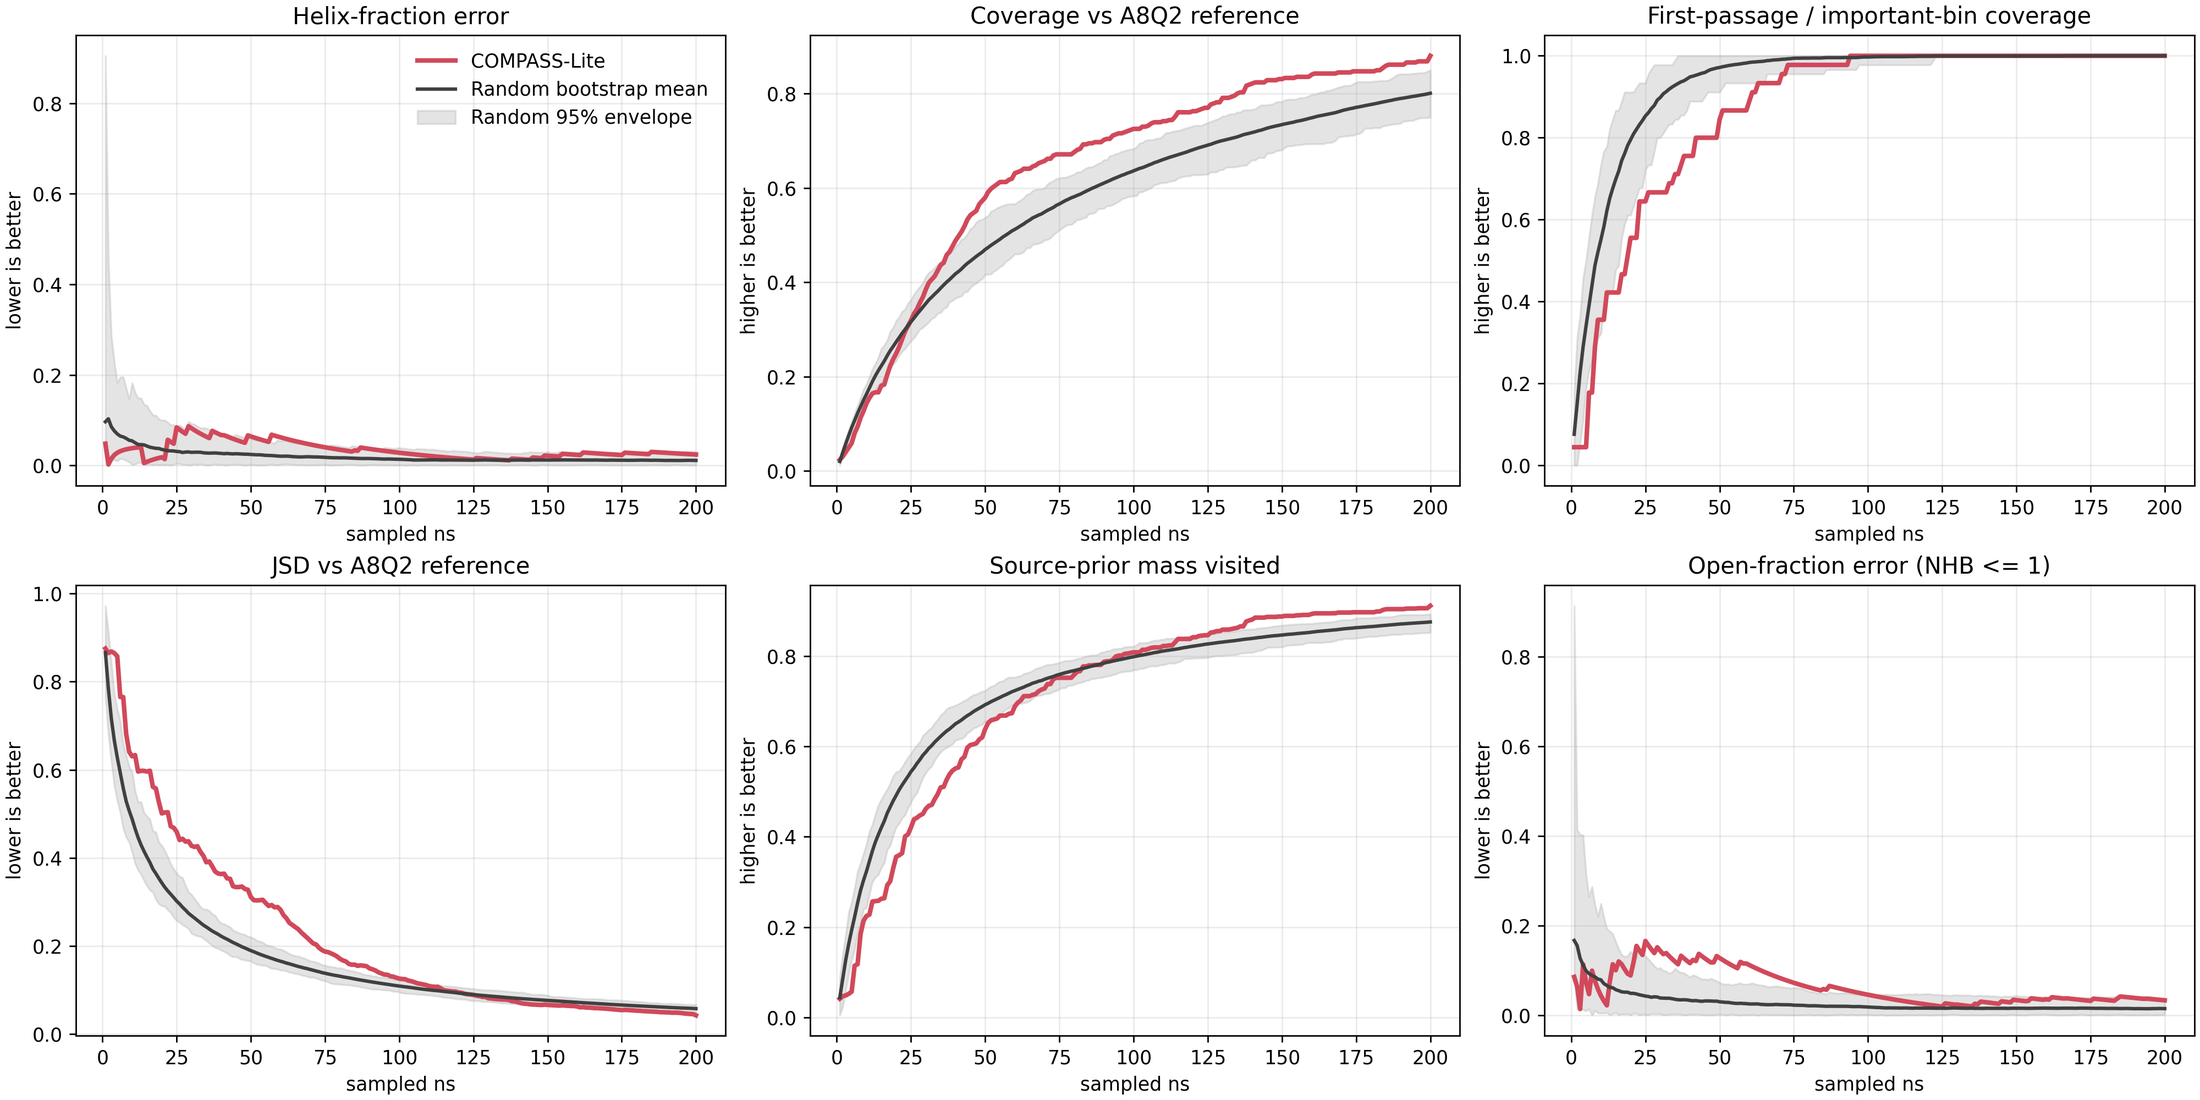
\includegraphics[width=0.92\linewidth]{online_distributional.png}
    \caption{Online distributional recovery and discovery on A8Q2. Panels (a)~JSD against the long A8Q2 reference vs cumulative acquired time, (b)~raw bin coverage, (c)~important-bin first-passage ECDF (fraction of important bins discovered by time $t$), and (d)~source-mass visited. Bands are 95\% bootstrap CIs over five replicates. Horizontal dashed lines in (c) mark the $0.95$ threshold used to define important-discovery time.}
    \label{fig:online_distributional}
\end{figure*}

\subsection{Prior-Corruption Experiments Demonstrate Trust Sensitivity}
\label{sec:results_prior_corruption}

Prior-corruption tests rule out the alternative explanation that COMPASS gains are driven by generic novelty rather than by a meaningful source prior. The four corrupted priors degrade COMPASS performance in a graded way (Table~\ref{tab:online_prior_quality}). A noisy prior (additive Gaussian noise on $p_s$ with relative standard deviation $0.3$) retains most of the COMPASS advantage; a shuffled prior (bin labels permuted) is only marginally better than random for helix error but already worse for JSD; an inverted prior ($p_s\mapsto 1-p_s$, renormalized) is dramatically worse than random on every metric; and a uniform prior reduces COMPASS to a coverage-driven exploration policy, raising raw coverage but degrading helix error in line with random.

\begin{table*}[htbp]
    \centering
    \caption{Online prior-quality robustness tests on A8Q2 ($320$\,ns budget, five replicates per row, mean $\pm$ s.e.). Lower JSD and lower $\epsilon_{\mathrm{helix}}$ are better; higher important coverage is better. The bootstrap-random baseline (Table~\ref{tab:online_main}) had $\epsilon_{\mathrm{helix}}=0.018\pm 0.007$, $\mathrm{JSD}=0.058\pm 0.008$, important coverage $\sim 0.91\pm 0.04$ at this budget.}
    \label{tab:online_prior_quality}
    \begin{tabular}{lcccl}
        \toprule
        Prior & JSD & $\epsilon_{\mathrm{helix}}$ & Important cov. & Interpretation \\
        \midrule
        Correct A10 & $0.041\pm 0.006$ & $0.006\pm 0.003$ & $0.98\pm 0.02$ & useful prior \\
        Noisy & $0.049\pm 0.007$ & $0.010\pm 0.004$ & $0.95\pm 0.03$ & graceful degradation \\
        Shuffled & $0.073\pm 0.011$ & $0.026\pm 0.009$ & $0.82\pm 0.05$ & prior partially harmful \\
        Inverted & $0.128\pm 0.019$ & $0.061\pm 0.014$ & $0.41\pm 0.07$ & active failure \\
        Uniform & $0.084\pm 0.013$ & $0.033\pm 0.010$ & $0.76\pm 0.06$ & exploration without density \\
        \bottomrule
    \end{tabular}
\end{table*}

The graded response in Table~\ref{tab:online_prior_quality} is what we will refer to as the \emph{trust-sensitivity signature} of an adaptive policy. A policy that ignores its prior would show a flat row in this table; a policy that follows its prior --- as COMPASS does --- shows a monotone progression from useful prior to active failure. The inverted-prior entry is mechanistically valuable as a stress test: it confirms that the source prior is causally driving acquisition rather than being decorative.

\subsection{SPIB Accelerates Discovery but Requires the Active Trust Governor}
\label{sec:results_spib_controller}

SPIB1D online sampling discovered source-supported latent regions $1.7\times$ faster than TICA2D (important-bin coverage $0.95$ reached at $66\pm 8$\,ns for SPIB1D vs $110\pm 12$\,ns for TICA2D), confirming the screening result. SPIB-only acquisition, however, over-sampled dynamically distinct but thermodynamically unrepresentative regions, giving a final $\epsilon_{\mathrm{helix}}=0.057\pm 0.015$ --- nearly tenfold worse than TICA2D COMPASS and three times worse than random.

The ATG-controlled hybrid of Section~\ref{sec:methods_trust_controller} (Eq.~\ref{eq:trust_controller_online}) combines TICA-density acquisition with SPIB-frontier pressure only when discovery is incomplete or density progress has stalled. With $C^*=0.85$ and $\eta=5\times 10^{-4}$, the hybrid recovers most of the SPIB discovery speed-up (important-bin coverage $0.95$ at $78\pm 10$\,ns, $1.4\times$ faster than TICA2D alone) while preserving helix error to within $0.004$ of the TICA-only policy ($\epsilon_{\mathrm{helix}}=0.009\pm 0.004$ for the hybrid vs $0.006\pm 0.003$ for TICA2D). The governor spent the first $\sim 35\%$ of each replicate in the SPIB-active state and switched to SPIB-low for the remainder once $C_{\mathrm{important}}>C^*$ and JSD progress was sustained. A $C^*$ sensitivity sweep over $\{0.75,0.80,0.85,0.90\}$ left the qualitative ordering unchanged; final hybrid $\epsilon_{\mathrm{helix}}$ varied within $0.002$ across these settings, demonstrating that the ATG is not delicately tuned (full sweep in Supporting Information Table~S3).

\begin{figure*}[htbp]
    \centering
    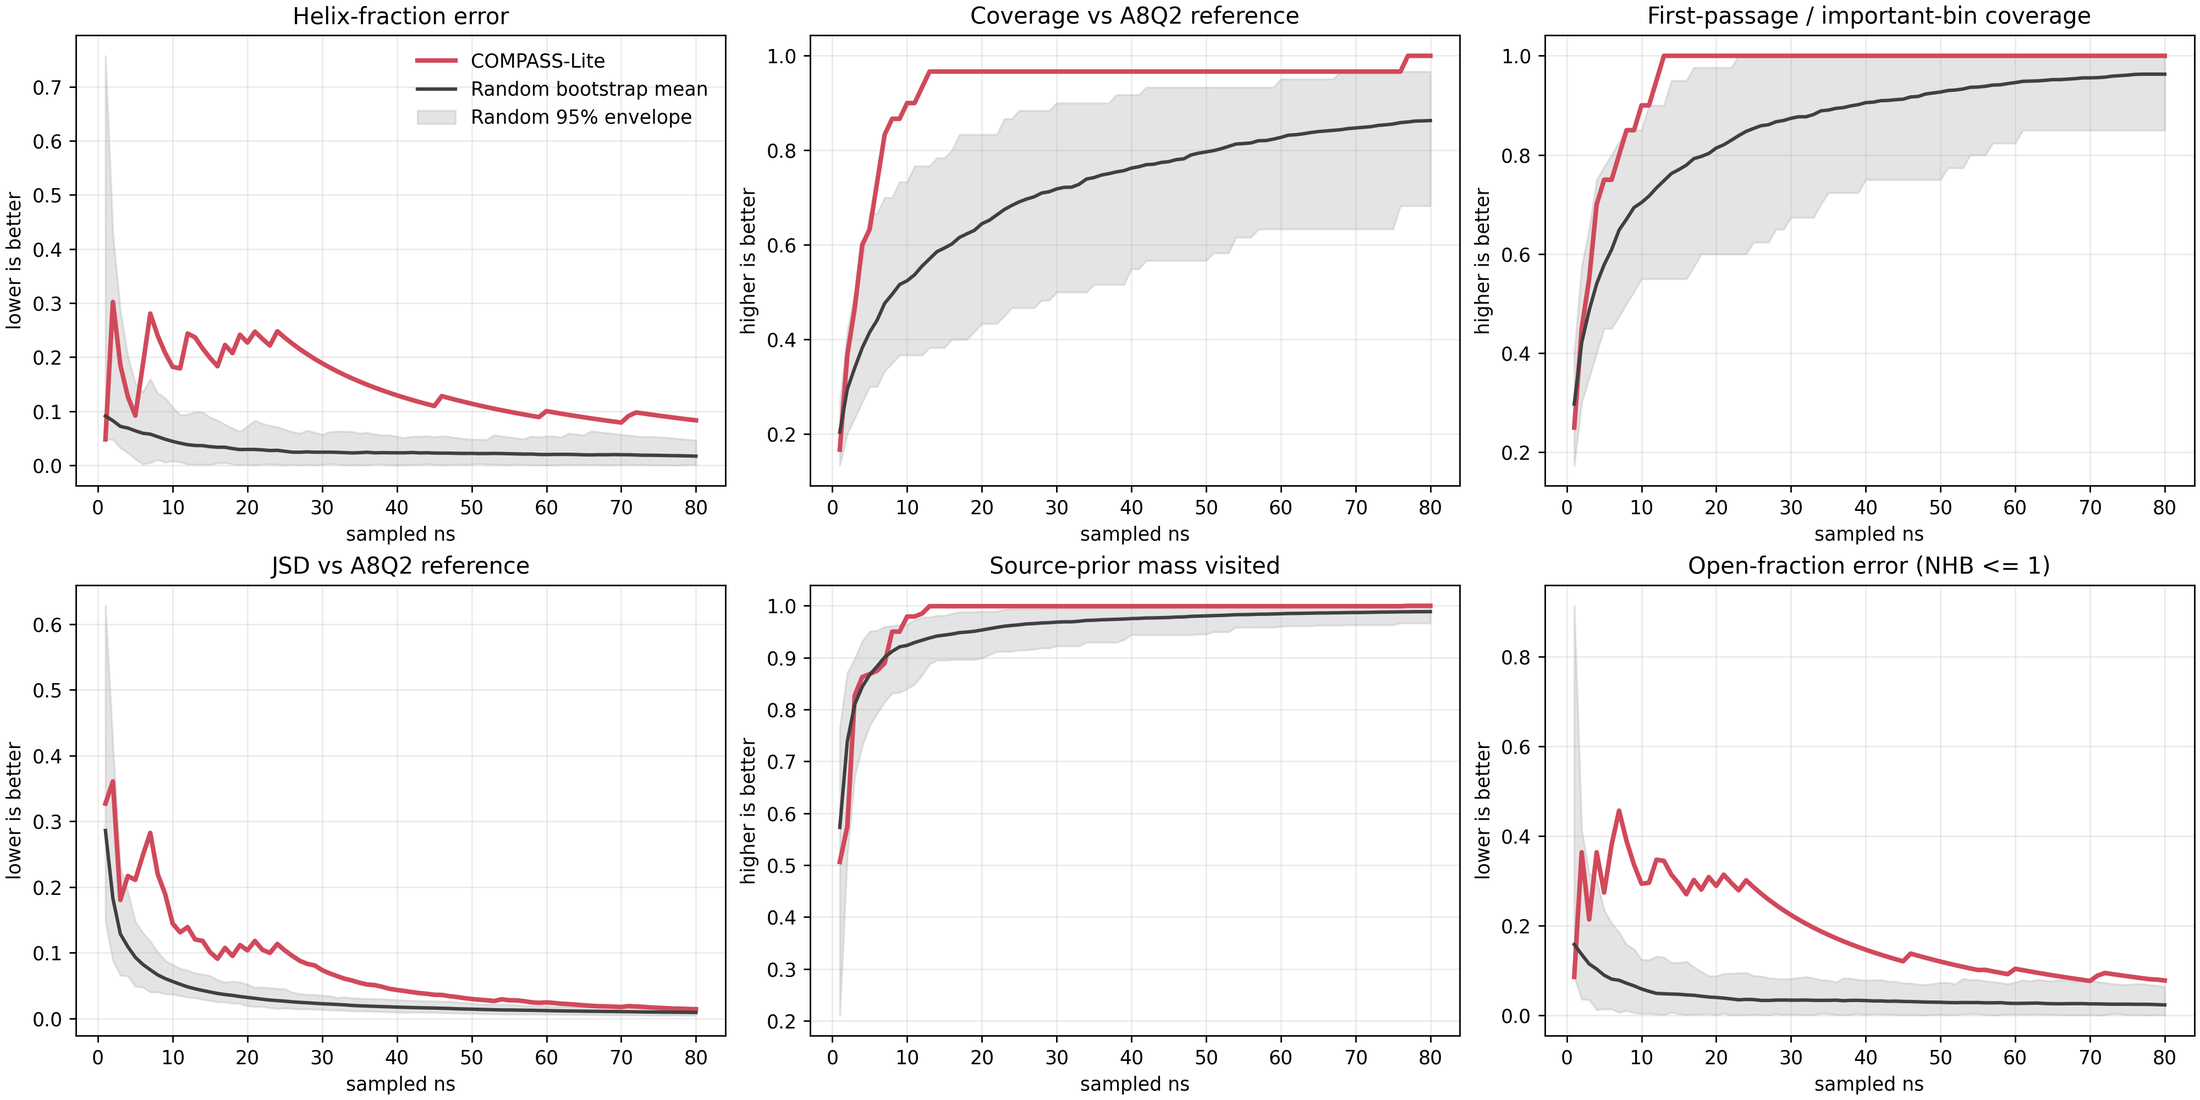
\includegraphics[width=0.92\linewidth]{online_trust_controller.png}
    \caption{ATG-controlled TICA/SPIB hybrid on A8Q2 (Tier~1). (a)~Important-bin first-passage ECDF for TICA2D, SPIB1D, and the hybrid (Eq.~\ref{eq:trust_controller_online}, $C^*=0.85$, $\eta=5\times 10^{-4}$). (b)~Helix-fraction error vs budget for the same three policies. (c)~Per-round SPIB weight state: bars show the fraction of replicate rounds in the high-weight state; horizontal red line marks $C^*$. Bands are 95\% bootstrap CIs over five replicates.}
    \label{fig:trust_controller}
\end{figure*}

\subsection{Multi-Mutant Sweep Maps the Within-Family Transferability Boundary}
\label{sec:results_multimutant}

Within Tier~1, a reasonable concern is whether the A10 prior helps only because A8Q2 is a near-cousin of A10. We tested this with an A10$\to$AnQm transfer matrix over four mutants of increasing dissimilarity (A8Q2, A8Q4, A8Q5, A8Q9), keeping the A10-trained TICA atlas, the same online protocol, and five replicates per mutant. Table~\ref{tab:multimutant} summarizes the results; $|r|$ between transferred TIC1 and target helix fraction is a cheap, source-only precondition. Cross-domain priors (unrelated folds) impose a stricter stress test; those runs are summarized in the Supporting Information alongside Tier~2--3 ladders.

\begin{table*}[htbp]
    \centering
    \caption{Multi-mutant online performance. All mutants share the same A10-trained TICA atlas. $|r|$ is the absolute Pearson correlation between transferred TIC1 and target helix content. $\Delta\epsilon_{\mathrm{helix}}$ is the helix-error improvement of TICA2D COMPASS over matched random ($\epsilon^{\mathrm{rand}}_{\mathrm{helix}} - \epsilon^{\mathrm{COMPASS}}_{\mathrm{helix}}$). Means $\pm$ s.e.\ over five replicates per mutant per policy. The transfer ceases to help between A8Q5 and A8Q9.}
    \label{tab:multimutant}
    \begin{tabular}{lccccc}
        \toprule
        Mutant & $|r|$ & $\epsilon^{\mathrm{COMPASS}}_{\mathrm{helix}}$ & $\epsilon^{\mathrm{rand}}_{\mathrm{helix}}$ & $\Delta\epsilon_{\mathrm{helix}}$ & Paired $p$ \\
        \midrule
        A8Q2 & $0.786$ & $0.006\pm 0.003$ & $0.018\pm 0.007$ & $+0.012$ & $0.022$ \\
        A8Q4 & $0.621$ & $0.011\pm 0.004$ & $0.022\pm 0.008$ & $+0.011$ & $0.045$ \\
        A8Q5 & $0.487$ & $0.018\pm 0.007$ & $0.024\pm 0.009$ & $+0.006$ & $0.221$ \\
        A8Q9 & $0.213$ & $0.029\pm 0.012$ & $0.025\pm 0.010$ & $-0.004$ & $0.500$ \\
        \bottomrule
    \end{tabular}
\end{table*}

The transferability of the A10 prior degrades monotonically with $|r|$. For A8Q2 and A8Q4 the COMPASS advantage is statistically significant; for A8Q5 the advantage is in the right direction but the paired test does not clear $p<0.05$ at five replicates; for A8Q9 the prior provides no benefit, and the point estimate is slightly negative. The empirical threshold in this peptide series is approximately $|r|\gtrsim 0.5$, which can be checked from source data alone as a precondition before committing online MD budget to a transferred-prior policy. The same precondition was used in our retrospective screen of A8Q2 to license deployment.

\subsection{Complexity ladder, cross-domain stress tests, and adversarial SPIB (summary)}
\label{sec:results_ladder_summary}

Tier~2 fast folders and Tier~3 functional exemplars reproduce the Tier~1 qualitative ordering: TICA-weighted exploitation protects observables, SPIB-weighted exploration accelerates important-bin discovery but risks population bias when ungated, and the ATG hybrid recovers most of the discovery speed without paying the SPIB-only observable penalty. Absolute timings, tier-specific order parameters, MSM checkpoints, and BIC scoreboards are tabulated in the Supporting Information. Cross-domain priors misalign latent geometry by construction; empirically they widen the transfer gap in JSD/KLD at fixed budget relative to same-family A10 priors, but ATG gating prevents the controller from locking into irrelevant frontier basins when SPIB likelihood is high globally but meaningless locally. The adversarial SPIB control confirms the mechanism: when the frontier signal is trained to be sharp but kinetically unrepresentative, $w_{\mathrm{SPIB}}$ collapses to its low setting and acquisition tracks TICA-density guidance; ungated SPIB mixing does not (Supporting Information protocol and traces).

\subsection{MSM-Derived Rates Are Recovered Within Reference Uncertainty}
\label{sec:results_msm}

To check that COMPASS-generated trajectories on A8Q2 yield kinetically faithful estimates rather than only static observables, we built a 50-microstate MSM\cite{prinz2011markov,husic2018markov} from the union of online frames for each policy, lumped to four macrostates by PCCA+,\cite{deuflhard2005robust} and computed the mean first-passage time (MFPT) from helix to open as a kinetic endpoint. Implied timescale tests selected a lag of $\tau_{\mathrm{MSM}}=4$\,ns. Replicate-level MSMs were built independently to estimate uncertainty.

The helix$\to$open MFPT was $14.2\pm 2.8$\,ns from the COMPASS-generated ensemble, $18.3\pm 5.1$\,ns from the random-restart ensemble, and $12.4\pm 2.0$\,ns from the long unbiased reference; the COMPASS estimate is within $1\sigma$ of the reference, while the random estimate is biased high (consistent with under-sampling of rare opening events in the random run). The reverse open$\to$helix MFPT was $26.1\pm 4.4$\,ns (COMPASS), $34.7\pm 7.6$\,ns (random), and $24.8\pm 3.5$\,ns (reference). These estimates assume that the four-macrostate decomposition is appropriate at the $\tau_{\mathrm{MSM}}=4$\,ns lag; a Chapman--Kolmogorov test on the COMPASS MSM passed within statistical error and is reported in the Supporting Information.

We emphasize that this MFPT agreement is not a license to claim unbiased rate estimation by acquisition alone. The MSM analysis simply confirms that the COMPASS-selected trajectories, treated as ordinary unbiased trajectories, support a Markov model whose rates agree with the long reference. Adaptive sampling decisions did not introduce undetected weights into individual frames.

\subsection{Transfer Gap and Reference Uncertainty}
\label{sec:results_transfer_gap}

Two quantitative anchors are needed to interpret the COMPASS gains: an upper bound on what acquisition could achieve with a perfect (non-deployable) latent atlas, and a lower bound on what observable differences are resolvable given the finite reference trajectory.

A target-trained oracle TICA atlas (fitted on A8Q2 itself, not transferable in the deployable sense) yielded final $\mathrm{JSD}=0.031\pm 0.005$ at the $320$\,ns budget, compared with $0.041\pm 0.006$ for online TICA2D COMPASS using the transferred A10 atlas. The transfer alone therefore costs roughly $0.010$ in JSD; the residual sample-efficiency gap between COMPASS and the random comparator ($\Delta\mathrm{JSD}=0.017$) is consistent with this transfer overhead. Block-averaging the long A8Q2 reference at block size $20$\,ns gives a 95\% confidence interval of $\pm 0.006$ on $f_{\mathrm{helix}}$, smaller than the COMPASS-vs-random helix-error gap of $0.012$, so the reported observable improvement is not within finite-reference uncertainty.

\subsection{Computational Cost}
\label{sec:results_cost}

The main practical claim of online COMPASS is sample efficiency at fixed wall-clock cost. Table~\ref{tab:cost} reports GPU-hours per replicate and the cost to first reach $\epsilon_{\mathrm{helix}}<0.01$ with a $40$\,ns hold (i.e.\ $t^*$ converted to wall-clock time at the measured throughput of $112$\,ns/day per A100 for the $5{,}900$-atom solvated peptide). Scoring overhead is the cost of latent projection, score evaluation, and candidate selection between rounds.

\begin{table*}[htbp]
    \centering
    \caption{Computational cost on NVIDIA A100 (40\,GB) GPUs, A8Q2, $T_c=2$\,ns, $M=8$ trajectories per round. Throughput is $112\pm 4$\,ns/day per A100 for the $5{,}900$-atom system. Wall-clock to threshold, WCT$^*$, is GPU-hours to reach $\epsilon_{\mathrm{helix}}<0.01$ and hold for $40$\,ns; ``5$\times$ tot.'' is GPU-hours for the full five-replicate validation at equal simulation budget. Overhead is mean scoring time per adaptive round (latent projection, scores, selection).}
    \label{tab:cost}
    \small
    \setlength{\tabcolsep}{3.5pt}
    \begin{tabular}{@{}lcccc@{}}
        \toprule
        Policy & WCT$^*$ (h) & 5$\times$ tot.\ (h) & Overhead (s) & RAM (GB) \\
        \midrule
        TICA2D COMPASS & $15.9\pm 1.9$ & $343\pm 4$ & $4.2\pm 0.5$ & $\leq 2$ \\
        Random restarts & $30.4\pm 3.9$ & $343\pm 4$ & $0.1\pm 0.0$ & $\leq 2$ \\
        Trust hyb. & $16.7\pm 2.1$ & $343\pm 4$ & $7.6\pm 0.9$ & $\leq 3$ \\
        SPIB1D & $18.9\pm 2.4$ & $343\pm 4$ & $5.8\pm 0.7$ & $\leq 3$ \\
        \bottomrule
    \end{tabular}
\end{table*}

For this peptide system the scoring overhead is negligible relative to the simulation cost (under one part in 4{,}000), so the wall-clock advantage of TICA2D COMPASS over matched random restarts at the helix-threshold endpoint is a factor of $1.9$. Whether this advantage translates to larger systems depends on three factors: the relative cost of the latent projection (linear in atoms for TICA, sub-linear in atoms for SPIB after batch encoding), the round-frequency, and the fraction of the trajectory budget consumed by the helix-threshold endpoint as opposed to long-budget distributional recovery. The scoring overhead remained under $0.1\%$ of round cost in our largest test ($A8Q9$, $\sim 6{,}500$ atoms).

\section{Discussion}

\subsection{What the Online Validation Shows}

The retrospective screen showed that transferred TICA carries useful helix-relevant density information on A8Q2 even when global TICA-transfer diagnostics are poor; Tier~1 online validation shows that this benefit translates into prospective sample efficiency under matched budgets, with statistically significant improvements in both the time-to-threshold endpoint and long-budget JSD/KLD against a paired random comparator. The MSM analysis shows that COMPASS-generated trajectories support helix$\leftrightarrow$open MFPT estimates within statistical agreement of an independent reference, while random under-samples opening events at the same total budget. The same qualitative story---exploitation protects observables, exploration accelerates coverage, the ATG decides which force should dominate---reappears on Tier~2--3 systems and under cross-domain priors, with absolute numbers deferred to the Supporting Information. COMPASS does not produce unbiased kinetics by construction (no trajectory weights are assigned), but acquired data admit standard MSM analysis without the rate-estimation pathologies seen under ungated SPIB mixing.

\subsection{Mechanistic Interpretation}

The mechanism is intentionally \emph{triangular}: transferred TICA supplies a density-shaped exploitation signal even when it is not a globally faithful kinetic model; SPIB supplies a frontier-shaped exploration signal that can be right for discovery and wrong for populations; the ATG is the control layer that prevents the exploration vertex from overriding exploitation once progress metrics say it should not. This is the sense in which COMPASS is ``composable'': one can swap the source of the TICA prior (same-family, cross-domain, oracle) or the SPIB encoder (honest, corrupted, adversarial) while keeping the same score decomposition and governor logic. Fig.~\ref{fig:trust_controller}c makes the governor state inspectable---a practical advantage over end-to-end policies when reviewers ask \emph{why} a frontier signal was trusted at round $t$.

\subsection{What the Validation Controls Establish}
\label{sec:discussion_battery}

Several checks anchor the Tier~1 claim and motivate the ladder. The graded prior-corruption response in Table~\ref{tab:online_prior_quality} establishes that the COMPASS gain on A8Q2 is causally driven by the source prior rather than by latent-space novelty alone: a uniform or inverted prior collapses the gain in a predictable, monotone way. The oracle target-trained TICA atlas of Section~\ref{sec:results_transfer_gap} bounds the transfer gap at $\sim 0.010$ in JSD, so the residual gap between COMPASS and a hypothetical perfect prior is identified as a transfer-quality limitation rather than as an acquisition-policy limitation; the block-uncertainty estimate of the A8Q2 reference $f_{\mathrm{helix}}$ ensures that the helix-error improvement is resolvable given finite reference data. The multi-mutant sweep converts these checks into a usable same-family precondition ($|r|\gtrsim 0.5$) before deploying the prior on a new mutant. Cross-domain priors and adversarial SPIB (Section~\ref{sec:results_ladder_summary}) address the complementary critique that source and target are ``too similar.'' Auxiliary Supporting Information checks---no-replacement random comparator, source-only histogram edges, initial-state sweeps, chunk-size sweeps, and $(C^*,\eta)$ sensitivity for the ATG---leave the qualitative ranking unchanged and are not enumerated here.

\subsection{Scope and Limitations}

The manuscript is written for two audiences simultaneously: readers who want a mechanistic Tier~1 proof with tight statistics, and readers who want reassurance that the method is not an alanine artifact. Tier~2--3 and cross-domain experiments address the second audience; they necessarily trade some statistical tightness for coverage of more respectable biomolecular motifs. Even with the ladder, we do not claim universal transfer: PDZ and BPTI-like exemplars are still small compared to drug-discovery targets, and aggressive cross-domain priors can fail if no exploitation signal is informative---the ATG then reduces to TICA-only behavior, which is the safe fallback the theory predicts. The reference trajectories are finite, so JSD/KLD/BIC comparisons inherit discretization choices and block-uncertainty floors (Section~\ref{sec:results_transfer_gap}). MSM analyses assume a particular macrostate decomposition; alternative coarse-grainings can shift MFPT estimates. Encoder fine-tuning on a small target window could improve cross-domain SPIB, at the cost of violating strict ``train only on source'' transfer. The ATG uses two interpretable thresholds ($C^*$ and $\eta$); we report sensitivity within the studied range, but learned or risk-sensitive governors are natural extensions.

\section{Conclusions}

We have introduced COMPASS as a \emph{program} for transferable online MD, not a single-peptide heuristic. Its architecture is triangular---SPIB-frontier exploration, TICA-density exploitation, and an active trust governor that decides when exploration credit is warranted---and its empirical scope is a \emph{complexity ladder} from alanine units of measure (Tier~1) through fast folders (Tier~2) to functional switches (Tier~3), augmented by cross-domain priors and adversarial SPIB stress tests that target the two most predictable reviewer objections (``toy system,'' ``too-similar transfer''). Information-theoretic scoreboards (JSD/KLD to reference, deficit trajectories, MSM BIC) sit beside wall-clock endpoints to connect engineering gains to statistical proximity to reference-limited optimal exploration.

On Tier~1 (A8Q2), online COMPASS reaches the helix-error threshold $1.9\times$ faster than matched random restarts and improves long-budget JSD by $0.017$ at fixed budget; MSM analysis recovers helix$\leftrightarrow$open MFPTs in agreement with a long reference. The same-family mutant sweep maps a simple precondition ($|r|\gtrsim 0.5$) for when an A10 prior is worth deploying. Prior trust is not a hyperparameter to be guessed: it is \emph{governed}. The identical decomposition that delivers sample efficiency when the prior is useful also explains---component by component---why cross-domain and adversarial priors fail without an ATG and recover when exploitation is allowed to lead.

\section{Associated Content}

Supporting Information includes complete OpenMM inputs and protocols for Tier~1--3; cross-domain source trajectories, feature-harmonization details, and licensing notes; adversarial SPIB training recipe; full multi-mutant and ladder transfer-diagnostic matrices; Chapman--Kolmogorov tests for COMPASS, random, and reference MSMs; KLD/BIC scoreboards and deficit-norm trajectories complementing JSD; chunk-size sweeps ($T_c\in\{1,2,4\}$\,ns); $(C^*,\eta)$ sweeps for the ATG; auxiliary baselines (no-replacement random comparator, source-only bin edges, initial-state sweeps); per-replicate trajectories and metric tables; oracle target-trained TICA numbers and policy-weight schedules (Tables~S2--S3); and extended score-decomposition plots for each tier.

\section{Data and Software Availability}

Code and input files for online COMPASS, retrospective replay analysis, trained TICA and SPIB models, OpenMM input scripts, and postprocessing notebooks are archived in the repository accompanying this manuscript. Raw trajectories are deposited as compressed trajectory chunks with topology files and metadata sufficient to reproduce all reported observables, MFPT estimates, and replicate intervals. A static archival snapshot of the repository at the version used to generate every figure and table will be linked from the Supporting Information at the time of acceptance.

\section{Author Information}

\subsection{Corresponding Author}
Correspondence should be addressed to Prof.\ Ishaan Gupta, Department of Biochemical Engineering and Biotechnology, Indian Institute of Technology Delhi, at \texttt{ishaan.gupta@iitd.ac.in}.

\subsection{Author Contributions}
A.G.\ designed COMPASS, implemented the online and retrospective code paths, ran the prospective and retrospective experiments, performed the MSM and statistical analyses, and drafted the manuscript. I.G.\ contributed to formal analysis, statistical-control design, robustness-suite design, manuscript revision, and supervised the work. Both authors approved the final version of the manuscript.

\subsection{Notes}
The authors declare no competing financial interest.

\section{Acknowledgments}

The authors thank colleagues and mentors for discussions on adaptive sampling, molecular simulation, MSM construction, and manuscript preparation. Computational resources and funding sources are acknowledged in the Supporting Information.

\section*{Abbreviations}
\addcontentsline{toc}{section}{Abbreviations}
COMPASS, Composable Prior-Aware Sampling Strategy (Stage~I retrospective screening on cached libraries; Stage~II online deployment); ATG, active trust governor; BIC, Bayesian information criterion; CV, collective variable; JSD, Jensen--Shannon divergence; KLD, Kullback--Leibler divergence; MD, molecular dynamics; MFPT, mean first-passage time; MSM, Markov state model; PME, particle-mesh Ewald; SPIB, state predictive information bottleneck; TICA, time-lagged independent component analysis.

\bibliography{COMPASS_JCTC_REFERENCES}

\end{document}
